\chapter{System do prowadzenia projektów}

Rozdział ten opisuje autorski system do prowadzenia projektów w trzech wersjach, każda z~nich różni się zastosowanym modelem i bazą danych.
Powstały dwie wersje odpowiednio dla baz Apache Cassandra i MongoDB, oraz trzeci wariant z modelem hybrydowym, gdzie część danych jest przechowywana w bazie relacyjnej, a część w bazie nierelacyjnej.
Główna część systemu powstała jako rezultat pracy inżynierskiej.
Niniejsza praca bazuje na nim rozszerzając nieznacznie jego funkcjonalność w celu dogłębniejszej analizy możliwości porównywanych baz.

\section{Specyfikacja wymagań funkcjonalnych}

Jedną z najważniejszych faz rozwoju oprogramowania jest wyspecyfikowanie wymagań.
Jest to część inżynierii oprogramowania dostarczająca nam środków i metod umożliwiających zebranie na temat funkcjonalności tworzonej przez nas aplikacji lub systemu komputerowego.
Popełnienie błędu w tej fazie projektu jest najbardziej kosztowne, ponieważ jest to początkowa faza i błędy w niej popełnione propagują się na kolejne fazy.

\subsection*{Role i uprawniania użytkowników w systemie}

W opisywanym systemie do prowadzenie projektów można wyróżnić następujące role i powiązane z nimi uprawnienia:
\begin{itemize}
    \item \textbf{Użytkownikiem} jest każdy, kto posiada zarejestrowane konto w aplikacji.
    \item \textbf{Administratorem projektu} staje się użytkownik aplikacji w momencie, gdy stworzy nowy projekt.
    Daje mu to uprawnienia do:
    \begin{itemize}
        \item dodawania nowych zadań w projekcie,
        \item usuwania istniejących zadań,
        \item usunięcia administrowanego projektu.
    \end{itemize}
    \item \textbf{Uczestnikiem zadania} staje się użytkownik, który został przypisany do zadania przez administratora.
    Dzięki temu zyskuje uprawnienia do:
    \begin{itemize}
        \item dodawania nowego pliku do zadania,
        \item pobrania wybranej wersji pliku,
        \item zaznaczenia pliku do zatwierdzenia przez administratora zadania,
        \item zapisania nowej wersji pliku,
        \item wyświetlenia szczegółowych informacji o wersji pliku.
    \end{itemize}
    \item \textbf{Administratorem zadania} zostaje użytkownik aplikacji, który został wybrany do tego przez administrator projektu podczas tworzenia zadania.
    Otrzymuje on wtedy następujące przywileje:
    \begin{itemize}
        \item możliwość przypisania/usunięcia uczestnika do/z administrowanego zadania,
        \item możliwość zatwierdzenia ostatecznej wersji pliku,
        \item możliwość usunięcia pliku.
    \end{itemize}
    Oprócz tych uprawnień użytkownik pełniący tą rolę otrzymuje wszystkie uprawniania uczestnika projektu.
\end{itemize}

Jeden użytkownik może pełnić wiele z wyżej wymienionych ról.
Pełniąc je dziedziczy wymienione uprawnienia. 

\subsection*{Przypadki użycia}

Przypadki użycia opisywanego systemu zostały podzielone na dwie grupy funkcjonalne.
Ma to na celu łatwiejsze zrozumienie oferowanej przez system funkcjonalności.

\subsubsection{Funkcjonalność związana z projektami i zadaniami}

Zbiór przypadków użycia związany z zarządzaniem projektami i zadaniami w systemie:
\begin{enumerate}
    \item \textbf{Utworzenie projektu} -- każdy użytkownik systemu może utworzyć i zarządzać swoimi projektami.
    \item \textbf{Wyświetlenie listy projektów}, w których uczestniczy użytkownik jest wyświetlane tuż po zalogowaniu się do aplikacji.
    \item \textbf{Wyświetlenie szczegółowych informacji o projekcie wraz z listą zadań} -- użytkownik może wyświetlić informacje o projekcie jeżeli jest uczestnikiem projektu tzn. jest administratorem projektu, lub administratorem lub uczestnikiem zadania.
    \item \textbf{Wyświetlenie szczegółowych informacji o zadaniu wraz z listą plików} -- użytkownik może wyświetlić informacje o zadaniu jeżeli jest przypisany do niego, lub jest jego administratorem.
    \item \textbf{Dodanie nowego zadania do projektu} -- uprawniony do tego jest administrator projektu.
    \item \textbf{Usunięcie zadania} -- uprawniony do tego jest administrator projektu.
    \item \textbf{Usunięcie projektu} -- uprawniony do tego jest administrator projektu.
    \item \textbf{Przypisanie nowego uczestnika do zadania} -- ta funkcja jest dostępna dla administratora zadania.
    \item \textbf{Usunięcie uczestnika z zadania} -- ta funkcja jest dostępna dla administratora zadania.
\end{enumerate}

\subsubsection{Funkcjonalność związana z plikami i ich wersjami}

Przypadki użycia związane z wszystkimi czynnościami, które można wykonać w~związku z~plikami w~obrębie systemu:
\begin{enumerate}
    \item \textbf{Wyszukiwanie pełnotekstowe wśród plików zadania/projektu} jest rozszerzeniem funkcjonalności systemu w porównaniu do systemu powstałego w pracy inżynierskiej.
    Ten przypadek użycia ma na celu zbadanie możliwości i wsparcia wyszukiwania pełnotekstowego przez bazy danych.
    Wyszukiwanie to jest dostępne dla uczestników projektów i zadań.
    Można je uruchomić z poziomu widoku listy zadań -- wtedy zostaną przeszukane wszystkie pliki zadań, do których użytkownik ma dostęp.
    Wyszukiwanie z widoku listy plików w zadaniu ogranicza przeszukiwane pliki do tych, które znajdują się w zadaniu.
    Po wyświetleniu listy plików dopasowanych do wyszukiwanej frazy można wybrać jeden z nich i przejść do szczegółowych informacji o nim.
    \item \textbf{Zatwierdzenie pliku} -- przypadek użycia przeznaczony dla administratora zadania. 
    Może być zrealizowany gdy system wyświetla listę plików przypisanych do zadania. 
    Po wybraniu pozycji z tej listy administrator wybiera opcję zatwierdzenia. 
    Po tej czynności plik posiada status zatwierdzony i nie może można go już edytować.
    \item  \textbf{Usunąć plik} może tylko administrator zadania. 
    Wraz z plikiem usuwane są wszystkie zapisane wersje. 
    W celu usunięcia pliku administrator wybiera pozycję z listy plików i~wybiera opcję usunięcia.
    \item \textbf{Wyświetlenie szczegółów pliku z listą wersji} -- uprawniony do tego jest uczestnik zadania.
    Może tego dokonać w poziomu widoku listy plików.
    \item \textbf{Dodanie nowego pliku} -- funkcjonalność dostępna dla każdego uczestnika zadania. 
    \item \textbf{Pobranie wersji pliku} -- dostępne dla uczestnika zadania. 
    Po przejściu do widoku listy wersji pliku może wybrać opcję pobrania konkretnej wersji.
    \item \textbf{Zaznaczenie pliku do zatwierdzenia przez administratora zadania} -- prosty przypadek użycia dostępny dla uczestnika zadania.
    Po wyświetleniu  szczegółowego widoku informacji o pliku może wybrać opcję oznaczenia pliku do zatwierdzania.
    \item \textbf{Zapisanie nowej wersji pliku} jest dostępne dla uczestnika zadania z poziomu widoku szczegółowych informacji o pliku.
    \item \textbf{Wyświetlenie szczegółowych informacji o wersji pliku} -- opcja dostępna dla uczestników zadania.
\end{enumerate}

\section{Architektura systemu}

System został zaprojektowany i zaimplementowany zgodnie z architekturą wielowarstwową jako aplikacja internetowa.
Składa się z dwóch aplikacji: klienta przeglądarkowego i serwera aplikacyjnego.
Można wyróżnić w nim następujące warstwy:
\begin{itemize}
    \item \textbf{warstwa dostępu do danych} -- nadaje poziom abstrakcji ukrywając technologię stojącą za przechowywaniem danych systemu.
    Na jej poziomie następują bezpośrednie połączenia z konkretną bazą danych i komunikacją z nią.
    Dzięki niej wymiana bazy danych sprowadza się do zmian we właśnie tej warstwie.
    \item \textbf{warstwa logiki biznesowej} -- odpowiedzialna za główną logikę aplikacji, koordynuje jej pracę. 
    Ponadto jest odpowiedzialna za przetwarzanie i przekazywanie danych między warstwą dostępu do danych, a warstwą kontrolerów.
    \item \textbf{warstwa kontrolerów} -- najbardziej zewnętrzna warstwa w serwerze aplikacyjnym, wystawia sieciowy interfejs programowania aplikacji (ang.~\textit{WebAPI}) dla klienta przeglądarkowego.
    Jest odpowiedzialna za przyjmowanie i odpowiadanie żądania od niego poprzez wywoływanie odpowiednich procedur warstwy logiki biznesowej.
    \item \textbf{warstwa prezentacji} -- klient przeglądarkowy, stanowi główny interfejs dla użytkownika systemu.
\end{itemize}

\section{Stos technologiczny}

\subsection*{Projekty platformy Spring}

Duży wpływ na końcową architekturę aplikacji miał szkielet aplikacyjnym Spring.
Obecnie Spring jest platformą open-source złożoną z wielu projektów, która dedykowana jest do tworzenia aplikacji w języku Java.
Jego głównym elementem jest kontener wstrzykiwania zależności (ang.~\textit{dependency injection container}).
Szkielet aplikacyjny Spring sam instancjonuje i zarządza zależnościami komponentów aplikacji.
Dzięki tym mechanizmom zostaje przeniesiona funkcja sterowania wykonywaniem programu do używanego frameworku (ang.~\textit{Inversion of Control}) -- Spring sam w odpowiednich momentach wywołuje kod stworzony w ramach implementacji aplikacji.
Posiada również bogate wsparcie dla aplikacji internetowych, dostępu do baz danych, integracji z~innymi systemami przez najpopularniejsze protokoły komunikacyjne oraz walidacji danych \cite{SpringReference}.

W aplikacji zostały wykorzystane następujące komponenty platformy Spring:
\begin{itemize}
    \item \textbf{Spring Framework} -- podstawowy moduł wiążący w jedną całość pozostałe elementy.
    \item \textbf{Spring Boot} -- jeden z najważniejszych modułów, zapewnia prostszy i szybszy sposób konfigurowania i uruchamiania aplikacji.
    \item \textbf{Spring WebMVC} -- moduł zawierający rozszerzenia niezbędne do stworzenia aplikacji internetowej.
    \item \textbf{Spring Security} -- szkielet aplikacyjny, który umożliwia twórcom aplikacji narzucanie ograniczeń dostępu w aplikacjach internetowych bazujących na stosie technologii Spring.
    Posiada wsparcie m. in. dla uwierzytelniania przez integrację z LDAP, autoryzacji tylko uwierzytelnionych żądań HTTP.
    \item \textbf{Spring Data} -- projekt zawierający wiele modułów dostarczających narzędzi dostępu do najpopularniejszych baz i źródeł danych. 
    Wszystkie te moduły mają wspólny cel, którym jest ukrycie mnogości i złożoności technologii przechowywania danych poprzez ujednolicenie i usystematyzowanie terminologii z nimi związanych do abstrakcyjnych, niezależnych od technologii pojęć.
    \item \textbf{Spring Test} -- zestaw narzędzi ułatwiających testowanie aplikacji wykorzystujących szkielet aplikacyjny Spring z wykorzystaniem wybranych bibliotek do testowania takich jak JUnit lub TestNG. 
\end{itemize}

\subsection*{Apache Tika}

Apache Tika jest biblioteką open-source wydaną przez Apache Software Foundation na licencji Apache License 2.0, dzięki czemu można używać jej zarówno w otwartym oprogramowaniu jaki i komercyjnym. 
Zaopatruje ona system w bogatą kolekcję parserów i detektorów dla znacznej liczby popularnych formatów plików.
Oprócz tego umożliwia odczyt wielu metadanych plików.
Dzięki detektorom nie trzeba znać odgórnie formatu parsowanego pliku co jest znaczącą zaletą tej biblioteki.
W omawianym w pracy systemie jest wykorzystywana do parsowania zapisywanych w aplikacji dokumentów.
Wydobyta w tej sposób zawartość jest później wykorzystywana do wyszukiwania pełnotekstowego wśród plików.

\subsection*{DiffUtils}

Biblioteka DiffUtils posłużyła do porównywania dwóch sparsowanych wersji plików.
W pierwszej kolejności odczytany tekst jest dzielony na wektory z liniami, z których następnie DiffUtils oblicza różnice, które są zapisywane do bazy danych.
Do wyznaczania różnic biblioteka ta domyślnie wykorzystuje implementację algorytmu stworzonego przez Eugene'a W. Myers'a.
Została ona napisana w całości w języku Java.
Podobnie jak Tika, narzędzie to jest udostępnione na licencji Apache 2.0.

\section{Model danych}

Omawiane wcześniej aspekty systemu do prowadzenia projektów były wspólne dla wszystkich trzech jego wersji, które zostały zaimplementowane.
Poniżej został opisany sposób w jaki zostały zaprojektowane i zaimplementowane warstwy dostępu do danych w poszczególnych wersjach.
Wykorzystanie modułów projektu Spring Data we wszystkich wersjach skróciło w znacznym stopniu czas pracy nad systemem.
W systemie można wyróżnić następujące encje i ich atrybuty, które zostały przełożone na odpowiednie struktury danych w danej technologii:
\begin{itemize}
    \item \textbf{Użytkownik} -- obiekt reprezentujący zarejestrowanego użytkownika aplikacji. 
    Składa się z pól:
    \begin{itemize}
        \item unikalny adres e-mail, które służy do m. in. logowania się,
        \item hasło, które służy do logowania się do aplikacji,
        \item wyświetlane w aplikacji imię i nazwisko użytkownika.
    \end{itemize}
    
    \item \textbf{Projekt} agreguje grupę zadań.
    Posiada nazwę, opis, datę utworzenia oraz przypisanego administratora.
    Może też posiadać 0 lub więcej zadań.
    
    \item \textbf{Zadanie} podobnie jak projekt posiada nazwę, opis, datę utworzenia i administratora.
    Zadanie posiada również przypisanych uczestników i pliki.
    
    \begin{samepage}
    \item \textbf{Plik} -- obiekt zawierający informację o przypisanym do zadania pliku i jego wersjach.
    Posiada następujące atrybuty:
    \begin{itemize}
        \item nazwa, która w kontekście zadania jest unikalna,
        \item opis,
        \item datę utworzenia pliku w systemie,
        \item flagę czy plik został oznaczony do zatwierdzenia,
        \item flagę informującą czy plik został zatwierdzony przed administratora zadania,
        \item wykryty format pliku.
    \end{itemize}
    \end{samepage}
    
    \item \textbf{Wersja} pliku niesie ze sobą informacje o zmianach dokonanych w pliku.
    Nie może istnieć bez pliku, do którego jest przypisana.
    Ma następujące pola:
    \begin{itemize}
        \item data zapisu,
        \item numer wersji, który jest wykorzystywany do identyfikowania jej wśród innych wersji tego samego pliku,
        \item wiadomość kontrolna autora modyfikacji informująca o dokonanych zmianach,
        \item suma kontrolna służąca do weryfikacji poprawności odczytu pliku i do szybkiego porównania czy nowa wersja jest rzeczywiście inna od poprzednich,
        \item autor, który zapisał wersję,
        \item lista zmian względem poprzedniej wersji,
        \item właściwy plik, który został przesłany w postaci binarnej -- może zostać pobrany z systemu przez innych uczestników zadania,
        \item sparsowana zawartość pliku w postaci tekstowej, która podlega analizie i indeksowaniu w celu możliwości przeszukiwania pełnotekstowego pliku.
    \end{itemize}
    
    \item \textbf{Zmiana} reprezentuje informacje o pojedynczej modyfikacji dokonanej w pliku.
    Zawiera następujące dane:
    \begin{itemize}
        \item początkowy wiersz z poprzedniej wersji pliku, który uległ zmianie,
        \item ilość wierszy, która uległa zmianie w poprzedniej wersji,
        \item początkowy wiersz w nowej wersji pliku, który reprezentuje zmianę,
        \item ilość wierszy, która została zmieniona w nowej wersji pliku,
        \item typ dokonanej zmiany.
    \end{itemize}
\end{itemize}

Rysunek \ref{fig:domainObjects} obrazuje wszystkie wymienione encje na diagramie UML.

\begin{figure}[!ht]
\centering
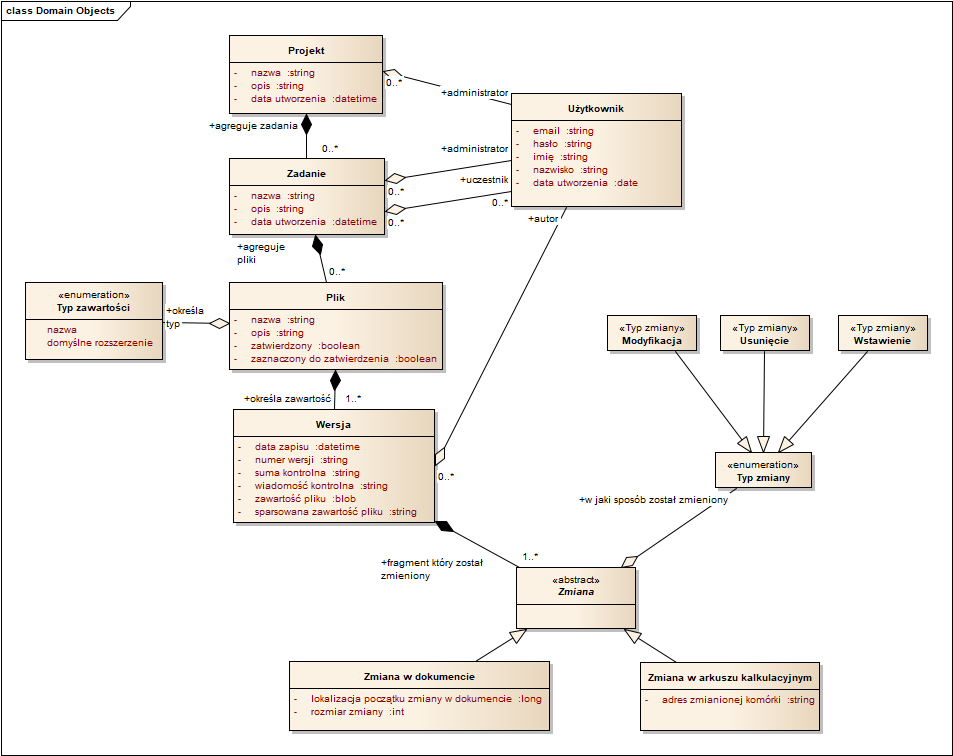
\includegraphics[width=\textwidth]{figures/domain_objects.png}
\caption{Model domenowy w opisywanym systemie}
\label{fig:domainObjects}
\end{figure}

\subsection{Apache Cassandra + Elasticsearch} \label{sec:ModelDanychCassandra}

Pierwsza z wersji systemu korzysta z modyfikacji bazy danych Apache Cassandra w wersji 3.11 zintegrowanej z wtyczką Elasticsearch w wersji 6.2.3 o nazwie Elassandra.
Z powodu braku operacji złączenia w zapytaniach do Cassandry i potrzeby obsługi tej czynności po stronie aplikacji, część danych wymagała denormalizacji w celu skrócenia czasu potrzebnego na ich odczyt.
Dodatkowej konfiguracji wymagało mapowanie indeksu wtyczki Elasticsearch na wybraną tabelę.

\subsubsection{Niestandardowe struktury danych} \label{sec:cassadnraUDFs}

Na potrzeby aplikacji powstały następujące niestandardowe typy danych, które zostały wykorzystane w definicjach tabel:
\begin{itemize}
    \begin{minipage}{\linewidth}
    \item \textbf{difference} -- struktura reprezentująca pojedynczą zmianę w dokumencie.
    Zawiera pola przedstawione na listingu \ref{lst:cassandraDifferenceUDT}
    \begin{lstlisting}[language=CQL,caption={Definicja niestandardowego typu \textit{difference}},label={lst:cassandraDifferenceUDT}]
CREATE TYPE difference (
    difference_type text,
    new_section_size bigint,
    new_section_start bigint,
    previous_section_size bigint,
    previous_section_start bigint
);
    \end{lstlisting}
    \end{minipage}
    
    \begin{minipage}{\linewidth}
    \item \textbf{user\_summary} -- typ przechowujący krótkie podsumowanie informacji o użytkowniku.
    Składa się z pól przedstawionych na listingu \ref{lst:cassandraUserSummaryUDT}.
    \begin{lstlisting}[language=CQL,caption={Definicja niestandardowego typu \textit{user\_summary}},label={lst:cassandraUserSummaryUDT}]
CREATE TYPE user_summary (
    email text,
    first_name text,
    last_name text
);
    \end{lstlisting}
    \end{minipage}
    
    \begin{minipage}{\linewidth}
    \item \textbf{file\_summary} -- struktura przechowująca krótkie podsumowanie informacji o pliku.
    Zawiera pola przedstawione na listingu \ref{lst:cassandraFileSummaryUDT}.
    \begin{lstlisting}[language=CQL,caption={Definicja niestandardowego typu \textit{file\_summary}},label={lst:cassandraFileSummaryUDT}]
CREATE TYPE file_summary (
    modification_author frozen<user_summary>,
    modification_date timestamp,
    name text,
    task_name text
);
    \end{lstlisting}
    \end{minipage}
    
    \begin{minipage}{\linewidth}
    \item \textbf{version\_summary} -- niestandardowy typ przechowujący krótkie podsumowanie informacji o wersji pliku.
    Składa się pól przedstawionych na listingu \ref{lst:cassandraVersionSummaryUDT}.
    \begin{lstlisting}[language=CQL,caption={Definicja niestandardowego typu \textit{version\_summary}},label={lst:cassandraVersionSummaryUDT}]
CREATE TYPE version_summary (
    modification_author frozen<user_summary>,
    save_date timestamp,
    version text
);
    \end{lstlisting}
    \end{minipage}
\end{itemize}

\subsubsection{Tabele}

Model danych stworzonej aplikacji obejmuje następujące tabele:
\begin{itemize}
    %% USER
    \item \textbf{user} -- tabela przechowująca dane o użytkownikach korzystających z systemu.
    Zawiera kolumny przedstawione na listingu \ref{lst:cassandraUserTable}.

    \begin{minipage}{\linewidth}
    \begin{lstlisting}[language=CQL,caption={Definicja tabeli \textit{user}},label={lst:cassandraUserTable}]
CREATE TABLE user (
    email text PRIMARY KEY,
    first_name text,
    last_name text,
    password text
);
    \end{lstlisting}
    \end{minipage}

    %% PROJECT
    \item \textbf{project} -- tabela przechowująca informacje o projektach.
    Zawiera kolumny przedstawione na listingu \ref{lst:cassandraProjectTable}.
    
    \begin{minipage}{\linewidth}
    \begin{lstlisting}[language=CQL,caption={Definicja tabeli \textit{project}},label={lst:cassandraProjectTable}]
CREATE TABLE project (
    id uuid PRIMARY KEY,
    administrator frozen<user_summary>,
    creation_date timestamp,
    description text,
    name text
);
    \end{lstlisting}
    \end{minipage}
    
    %% USER_PROJECT
    \item \textbf{user\_project} -- specjalna tabela przechowująca relację uczestnik projektu -- projekt. 
    Powstała w celu szybkiej weryfikacji czy dany użytkownik jest uczestnikiem projektu.
    Oprócz identyfikatorów użytkownika i projektu tabela zawiera informacje podsumowujące projekt, które są widoczne na listingu \ref{lst:cassandraUserProjectTable}. 
    Dane te są wyświetlane na liście projektów widocznej tuż po zalogowaniu do systemu.
    Powstała redundancja jest jednak rekompensowana szybkością operacji odczytu danych.
    
    \begin{minipage}{\linewidth}
    \begin{lstlisting}[language=CQL,caption={Definicja tabeli \textit{user\_project}},label={lst:cassandraUserProjectTable}]
CREATE TABLE user_project (
    user_email text,
    project_id uuid,
    creation_date timestamp,
    last_modified_file frozen<file_summary>,
    name text,
    number_of_files bigint,
    number_of_participants bigint,
    number_of_tasks bigint,
    PRIMARY KEY (user_email, project_id)
) WITH CLUSTERING ORDER BY (project_id ASC);
    \end{lstlisting}
    \end{minipage}
    
    %% TASK
    \item \textbf{task} -- tabela przechowująca dane o zadaniach w systemie.
    Składa się z kolumn przedstawionych na listingu \ref{lst:cassandraTaskTable}.
    Klucz główny jest złożony z kolumn \textit{project\_id} i \textit{task\_id}. 
    Kolumna \textit{project\_id} jest kluczem partycjonującym co zapewnia, że dane o zadaniach z jednego projektu będą przetrzymywane w jednym węźle.
    Kluczem sortującym dane w partycji jest kolumna \textit{task\_id}.
    
    \begin{minipage}{\linewidth}
    \begin{lstlisting}[language=CQL,caption={Definicja tabeli \textit{task}},label={lst:cassandraTaskTable}]
CREATE TABLE task (
    project_id uuid,
    task_id uuid,
    administrator frozen<user_summary>,
    creation_date timestamp,
    description text,
    last_modified_file frozen<file_summary>,
    name text,
    number_of_files bigint,
    participants set<frozen<user_summary>>,
    PRIMARY KEY (project_id, task_id)
) WITH CLUSTERING ORDER BY (task_id ASC);
    \end{lstlisting}
    \end{minipage}
    
    \item \textbf{file\_metadata} -- tabela przechowująca dane o plikach zapisanych w systemie.
    Składa się z kolumn przedstawionych na listingu \ref{lst:cassandraFileMetadataTable}.
    Kluczem partycjonującym jest kolumna \textit{task\_id}, przez co informacje o plikach z jednego zadania są przechowywane na jednym węźle klastra.
    Dane w pojedynczej partycji są posortowane rosnąco według wartości w kolumnie \textit{file\_id}.
    
    \begin{minipage}{\linewidth}
    \begin{lstlisting}[language=CQL,caption={Definicja tabeli \textit{file\_metadata}},label={lst:cassandraFileMetadataTable}]
CREATE TABLE file_metadata (
    task_id uuid,
    file_id uuid,
    confirmed boolean,
    content_type text,
    creation_date timestamp,
    description text,
    latest_version frozen<version_summary>,
    marked_to_confirm boolean,
    name text,
    number_of_versions bigint,
    task_name text,
    PRIMARY KEY (task_id, file_id)
) WITH CLUSTERING ORDER BY (file_id ASC);
    \end{lstlisting}
    \end{minipage}
    
    \item \textbf{version} -- w tej tabeli przechowywane są dane o pojedynczej wersji pliku, wliczając w~to informacje o autorze modyfikacji, listę różnic względem poprzedniej wersji i zawartość pliku.
    Wszystkie kolumny składające się na tabele są wypisane na listingu \ref{lst:cassandraVersionTable}.
    Kluczem partycjonującym jest kolumna \textit{file\_id}, a dane są posortowane w odwrotnym porządku chronologicznym według kolumny \textit{save\_date}, przez co wyszukanie najnowszej wersji pliku, lub wybór wersji z danego przedziału czasowego jest bardzo szybki.
    
    \begin{minipage}{\linewidth}
    \begin{lstlisting}[language=CQL,caption={Definicja tabeli \textit{version}},label={lst:cassandraVersionTable}]
CREATE TABLE version (
    file_id uuid,
    save_date timestamp,
    author frozen<user_summary>,
    check_sum text,
    differences list<frozen<difference>>,
    file_content blob,
    message text,
    parsed_file_content text,
    version_string text,
    PRIMARY KEY (file_id, save_date)
) WITH CLUSTERING ORDER BY (save_date DESC);
    \end{lstlisting}
    \end{minipage}
\end{itemize}

\subsubsection{Konfiguracja indeksowania tekstowego} \label{sec:cassandraTextIndexConfig}

W celu wyszukiwania pełnotekstowego zawartości plików indeksowaniu przez wtyczkę Elasticsearch podlegała tylko tabela \textit{version},
a dokładnie jej kolumny:
\begin{itemize}
    \item \textit{file\_id} -- identyfikator pliku,
    \item \textit{save\_date} -- data zapisu wersji,
    \item \textit{version\_string} -- wprowadzony przez autora numer wersji,
    \item \textit{message} -- wiadomość kontrolna,
    \item \textit{parsed\_file\_content} -- sparsowana zawartość pliku.
\end{itemize}

\subsection{MongoDB}

Druga wersja systemu korzysta z bazy danych MongoDB w wersji 4.0.
Wszystkie powiązania do dokumentów, które są w innych kolekcjach zostały zaimplementowane z pomocą odwołania typu \textit{DBRef}, które zostały dokładniej opisane w sekcji \ref{sec:MongoModelDanych} na stronie \pageref{sec:MongoModelDanych}.
Dzięki temu dołączona do aplikacji biblioteka \textit{Spring Data for MongoDB} pobiera, gdy to jest potrzebne, powiązane dokumenty. 
Każda, niżej wymieniona, kolekcja przechowuje zserializowane obiekty odpowiadającej jej klasy w aplikacji.

Model danych aplikacji obejmuje następujące kolekcje:
\begin{itemize}
    \item \textbf{user} -- kolekcja przechowująca informacje o zarejestrowanych użytkownikach.

    \item \textbf{project} -- kolekcja przechowująca dokumenty z informacjami o projektach.
    W celach wydajnościowych mogą one zawierać również powiązanie z ostatnio modyfikowanym plikiem oraz informacje o liczbie plików, zadań i uczestników w projekcie.
    
    \item \textbf{task} -- kolekcja przechowująca dokumenty z informacjami o zadaniach.
    Zawierają one pole z odwołaniem do projektów, do których są przypisane, oraz pole z odwołaniem do ostatnio modyfikowanego pliku.
    Relacja \textit{zadanie -- uczestnicy zadania} została zrealizowana za pomocą listy osadzonych dokumentów.
    
    \item \textbf{fileMetadata} -- kolekcja przechowująca dokumenty z metadanymi plików.
    Oprócz pól zdefiniowanych w encji pliku dokumenty posiadają odwołania do zadań, do których są przypisane.
    Dodatkowo posiadają również pole z referencją do najnowszej wersji pliku.
    
    \item \textbf{version} -- kolekcja przechowująca dokumenty z informacjami o wersjach plików.
    Posiada dodatkowy indeks na polu przechowującym datę zapisu wersji w celu szybszego odczytu najnowszej wersji pliku.
    Pola ze sparsowaną zawartością pliku i wiadomością kontrolną autora podlegają indeksowaniu pełnotekstowemu.
\end{itemize}

\subsection{Model hybrydowy}

Trzecia wersja systemu bazuje na modelu hybrydowym -- dane \enquote{relacyjne} są przechowywane w bazie PostgreSQL 10, a krytyczne dla działania i wydajności systemu dane są przechowywane w bazie Apache Cassandra 3.11, wspomnianej w sekcji \ref{sec:ModelDanychCassandra}.

Przez dane krytyczne dla działania i wydajności systemu przyjęto informacje o wersjach plików, które mogą być najczęściej czytane, dodawane i modyfikowane przez użytkowników aplikacji.

\subsubsection{Część relacyjna}

Część relacyjna modelu hybrydowego działa w oparciu o bazę PostgreSQL 10, która jest jedną z najpopularniejszych i najbardziej dojrzałym darmowym rozwiązań wśród baz relacyjnych.
Ta część modelu powstała w oparciu o model domeny.
Na podstawie klas i ich atrybutów zostały zaprojektowane tabele.
Diagram przedstawiający ten fragment modelu znajduje się na rysunku~\ref{fig:postgreModelDiag}.

\begin{figure}[!ht]
\centering
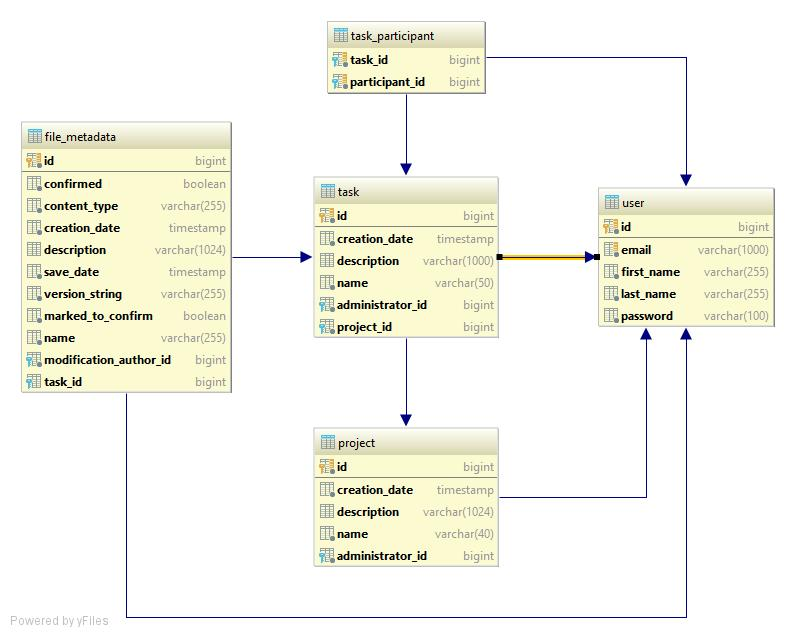
\includegraphics[width=0.8\textwidth]{figures/diagram.jpg}
\caption{Część relacyjna modelu hybrydowego}
\label{fig:postgreModelDiag}
\end{figure}

W tej części modelu możemy wyróżnić następujące tabele:
\begin{itemize}
    \item \textbf{Tabela użytkowników -- user} \\ 
    Posiada dwa indeksy w celu przyspieszenia wyszukiwania użytkowników -- jeden na kluczu głównym, a drugi na kolumnie \textit{email}.
    
    \item \textbf{Tabela projektów -- project} \\
    Zawiera klucz obcy odnoszący się do rekordu w tabeli \textit{user}. 
    Identyfikuje on administratora projektu.
    
    \item \textbf{Tabela zadań -- task} \\
    Zawiera klucz obcy odnoszący się do administratora zadania, oraz klucz do projektu, do którego zadanie jest przypisane.
    
    \item \textbf{Tabela asocjacyjna -- task\_participant} \\
    Tworzy relację wiele do wielu pomiędzy uczestnikami zadania i zadaniami, w których użytkownik bierze udział. 
    Posiada dwa kolumny, które są jednocześnie kluczami obcymi do tabel zadań i użytkowników. 
    Wpisy nie mogą zawierać pustych wartości, oraz nie mogą się duplikować przez nałożenie unikalności na każdy wiersz.
    
    \item \textbf{Tabela metadanych plików -- file\_metadata} \\
    Przechowuje klucz obcy do zadania, do którego jest przypisany plik.
    Posiada nałożone ograniczenie na unikalność par wartości \textit{name} i \textit{task\_id}, aby nazwy plików nie powtarzały się w tym samym zadaniu.
\end{itemize}

\subsubsection{Część nierelacyjna}

Część nierelacyjna oparta na Cassandrze 3.11 z wtyczką Elasticsearch 6.3.2 składa się jednej tabeli o nazwie \textit{version}.
Używa ona niestandardowych struktur danych, których definicje zostały opisane w sekcji \ref{sec:cassadnraUDFs} na stronie \pageref{sec:cassadnraUDFs}.
Różni się ona od tabeli \textit{version} z modelu bazującego w~całości na Cassandrze tym, że kolumna \textit{file\_id} jest typu \textit{bigint}.
Ma to na celu przechowywanie identyfikatorów plików, które w bazie PostgreSQL są liczbami całkowitymi.
Definicja tabeli \textit{version} została przedstawiona na listingu \ref{lst:cassandraHybridVersionTable}.

\begin{minipage}{\linewidth}
\begin{lstlisting}[language=CQL,caption={Definicja tabeli \textit{version} w modelu hybrydowym},label={lst:cassandraHybridVersionTable}]
CREATE TABLE version (
    file_id bigint,
    save_date timestamp,
    author frozen<user_summary>,
    check_sum text,
    differences list<frozen<difference>>,
    file_content blob,
    message text,
    parsed_file_content text,
    version_string text,
    PRIMARY KEY (file_id, save_date)
) WITH CLUSTERING ORDER BY (save_date DESC)
\end{lstlisting}
\end{minipage}

Konfiguracja indeksowania pełnotekstowego przez wtyczkę Elasticsearch pozostaje również identyczna co modelu bazującym tylko na samej Cassandrze i została ona opisana na stronie~\pageref{sec:cassandraTextIndexConfig} niniejszej pracy.
